\documentclass[aspectratio=169]{beamer}
% Pacote de estilo da UDESC
\usepackage{style/udesc}
\usepackage{listings}
\usepackage{hyperref}
\setbeamertemplate{itemize items}[circle]
\usepackage[abnt-emphasize=bf,abnt-and-type=e,alf]{abntex2cite}%Citações ABNT


% Incluir arquivos da pasta figuras
\graphicspath{{./img/}}

\setbeamertemplate{frametitle continuation}{}

% aPacote de texto aleatório
\usepackage{lipsum}

\lstset{ 
	basicstyle=\footnotesize,        % the size of the fonts that are used for the code
	breakatwhitespace=false,         % sets if automatic breaks should only happen at whitespace
	breaklines=true,                 % sets automatic line breaking
	captionpos=b,                    % sets the caption-position to bottom
	deletekeywords={...},            % if you want to delete keywords from the given language
	escapeinside={\%*}{*)},          % if you want to add LaTeX within your code
	extendedchars=true,              % lets you use non-ASCII characters; for 8-bits encodings only, does not work with UTF-8
	firstnumber=0,                % start line enumeration with line 1000
	frame=single,	                   % adds a frame around the code
	keepspaces=true,                 % keeps spaces in text, useful for keeping indentation of code (possibly needs columns=flexible)
	language=Java,                 % the language of the code
	morekeywords={*,...},            % if you want to add more keywords to the set
	numbers=none,                    % where to put the line-numbers; possible values are (none, left, right)
	numbersep=0pt,                   % how far the line-numbers are from the code
	rulecolor=\color{black},         % if not set, the frame-color may be changed on line-breaks within not-black text (e.g. comments (green here))
	showspaces=false,                % show spaces everywhere adding particular underscores; it overrides 'showstringspaces'
	showstringspaces=false,          % underline spaces within strings only
	showtabs=false,                  % show tabs within strings adding particular underscores
	stepnumber=2,                    % the step between two line-numbers. If it's 1, each line will be numbered
	tabsize=1,	                   % sets default tabsize to 2 
	basicstyle=\fontsize{7}{8}\selectfont\ttstyle,
	keywordstyle=\color{blue},
	commentstyle=\fontsize{7}{8}\selectfont\ttstyle\color{gray},
	stringstyle=\color{orange},
}

% Início do documento
\begin{document}
\usetikzlibrary{positioning}
\usetikzlibrary{shadows.blur, trees}
\definecolor{greenudesc}{HTML}{01934A}
\usepgfmodule{animations}

%%
%%	Incluir \capa para os slides
%% 
\titulo{Estágio Curricular -- IV}
\subtitulo{EEB. Giovai Pasqualini Faraco}
\newcommand{\autor}{Rodrigo Nascimento}
\newcommand{\github}{github.com/physikices}
\newcommand{\email}{rodrigo.nascimento@edu.udesc.br}
\newcommand{\website}{}
\frase{2023 - ESC4003}
\universidade{Licenciatura em Física\\Universidade do Estado de Santa Catarina}
\capa

\AtBeginSection[]{
	\begin{frame}<beamer>
		\frametitle{Seções}
		\tableofcontents[currentsection]
\end{frame}}

\section{Introdução}
\subsection{Objetivos}
\subsection{Apresentação da Concedente}
\subsection{Infraestrutura}

\section{Atividades de Observação}
\subsection{Acompanhamento de Aulas}
\subsection{Reuniões Pedagógicas}

\section{Atividades de Regência}
\subsection{Perfil da Turma}
\subsection{A Trilha/Tema}
\subsection{Planejamento}
\subsection{Análises}

\section{Considerações Finais}
% --------------------------------------------- %
% INÍCIO
% --------------------------------------------- %
% --------------------------------------------- %
% Introdução
% --------------------------------------------- %
\begin{frame}[plain]
	\tikzset{
		udesc greenBox/.style = {
			thin,
			blur shadow={
				shadow blur steps=10,
				shadow blur extra rounding=2pt, 
				shadow xshift=1pt
			},
			rectangle,
			minimum width=14em,
			minimum height=20mm,
			fill=greenudesc,
			text centered,
			anchor=base,
			inner sep=2ex
		},
	}
	\begin{tikzpicture}[remember picture,overlay]
		\node
			[udesc greenBox,yshift=-25pt,xshift=20pt] (box){}; 
		\node [right of = box, align=right,text=white] { {\LARGE Introdução}\\Objetivos};
	\end{tikzpicture}
\end{frame}
\begin{frame}{Introdução}
	\framesubtitle{Objetivos}
	\begin{columns}
		\column{0.5\textwidth}
		\begin{itemize}
			\item<1-> \textcolor<1>{olive}{Observar} rotinas próprias do ambiente de trabalho (gestão, relações de trabalho, organização etc.);
			\item<2-> \textcolor<2>{olive}{Perceber} o uso de metodologias/estratégias de Ensino;
			\item<3-> \textcolor<3>{olive}{Experienciar} situações próprias do cotidiano do trabalho.
		\end{itemize}

		\column{0.5\textwidth}
		\begin{figure}[htb!]
			\centering
			\only<1>{
				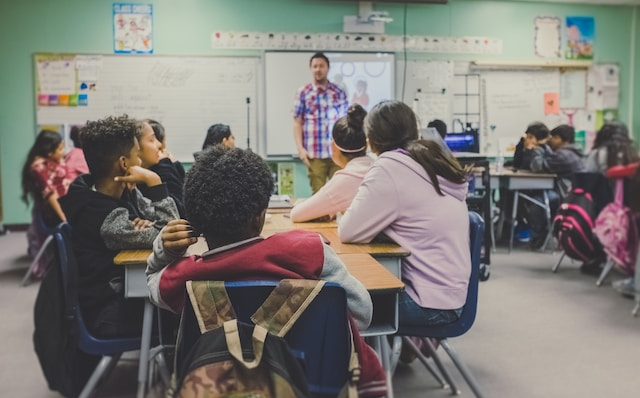
\includegraphics[width=1\linewidth]{introducao-rotina.jpg}
			}
			\only<2>{
				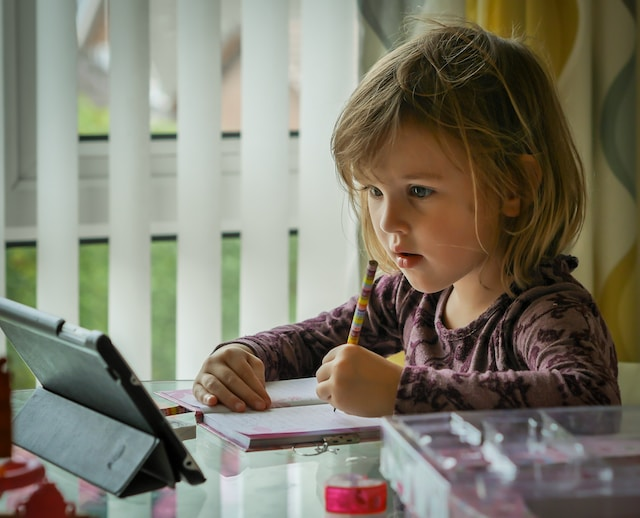
\includegraphics[width=1\linewidth]{introducao-metodologia.jpg}
			}
			\only<3>{
				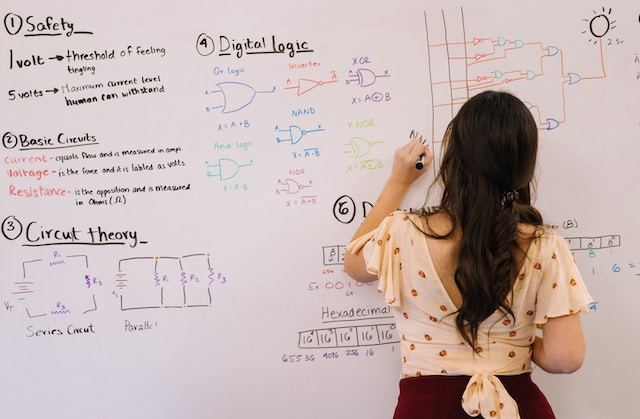
\includegraphics[width=1\linewidth]{introducao-experienciar.jpg}
			}
		\end{figure}
	\end{columns}
\end{frame}

\begin{frame}{Introdução}
	\framesubtitle{Apresentação da Concedente}
	\begin{columns}
		\column{0.5\textwidth}
		\only<1->{
			\only<1>{
				\begin{center}
					\textcolor{greenudesc!100!black!100}{Escola Desdobrada D. Francisca Km 5}

					\textcolor{olive}{Ano de Fundação}
				\end{center}
			}
			\only<2->{
				\begin{center}
					\textcolor{greenudesc!100!black!100}{EEB. Giovani Pasqualini Faraco -- (GPF)}

					\only<2>{\textcolor{olive}{Ano de Renomeação}}
					\only<3>{\textcolor{olive}{Localização -- Norte}}
					\only<4>{\textcolor{olive}{Qtde de Alunos/Turmas}}
				\end{center}
			}
		}
		\begin{itemize}
			\item<1-> 15/02/19\textcolor<1>{olive}{38} \textcolor<1>{olive}{(85 anos)}
			\item<2-> Decreto \textcolor<2>{olive}{10138/70}
			\item<3-> R. Dona Francisca, 4957 -- \textcolor<3>{olive}{Santo Antônio/Jlle-SC}
			\item<4-> Total \textcolor<4>{olive}{1165 Alunos}
		\end{itemize}

		\column{0.5\textwidth}
		\begin{figure}[htb!]
			\centering
			\only<1>{
				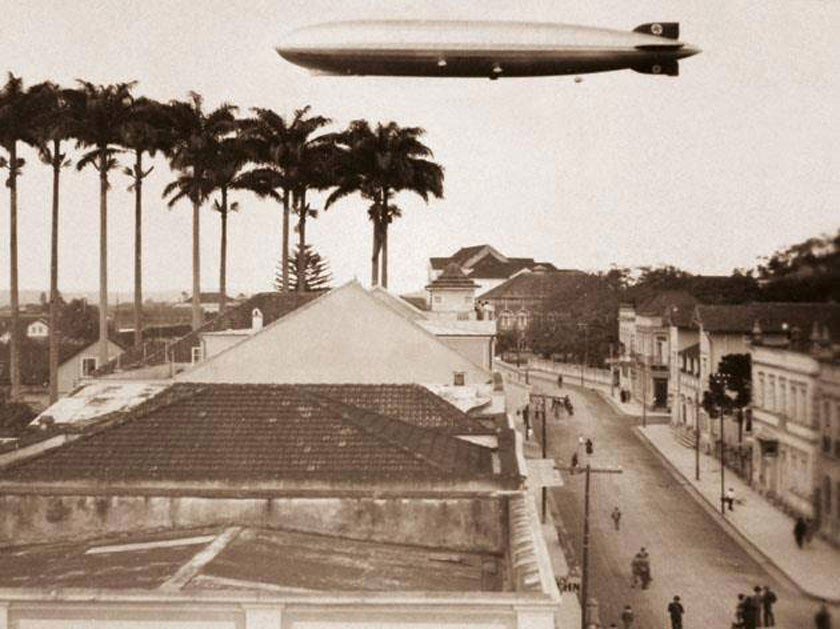
\includegraphics[width=\linewidth]{img/introducao-zeppelin.jpg}
				\caption{Hindenburg -- 1936}
			}
			\only<2>{
				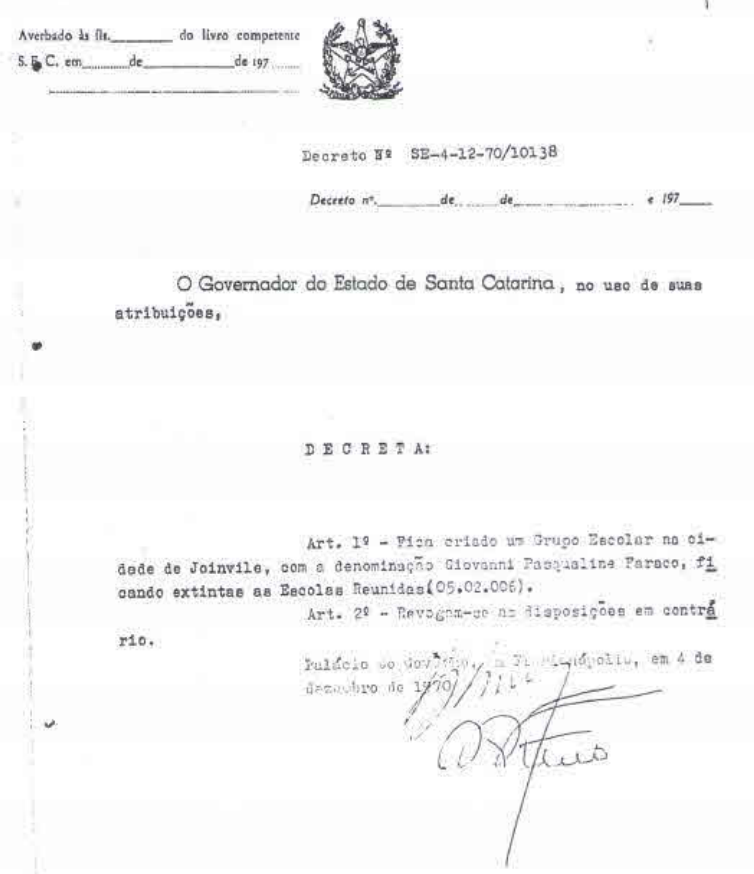
\includegraphics[width=.7\linewidth]{img/introducao-fundacao}
				\caption{Decreto -- 1970}
			}
			\only<3>{
				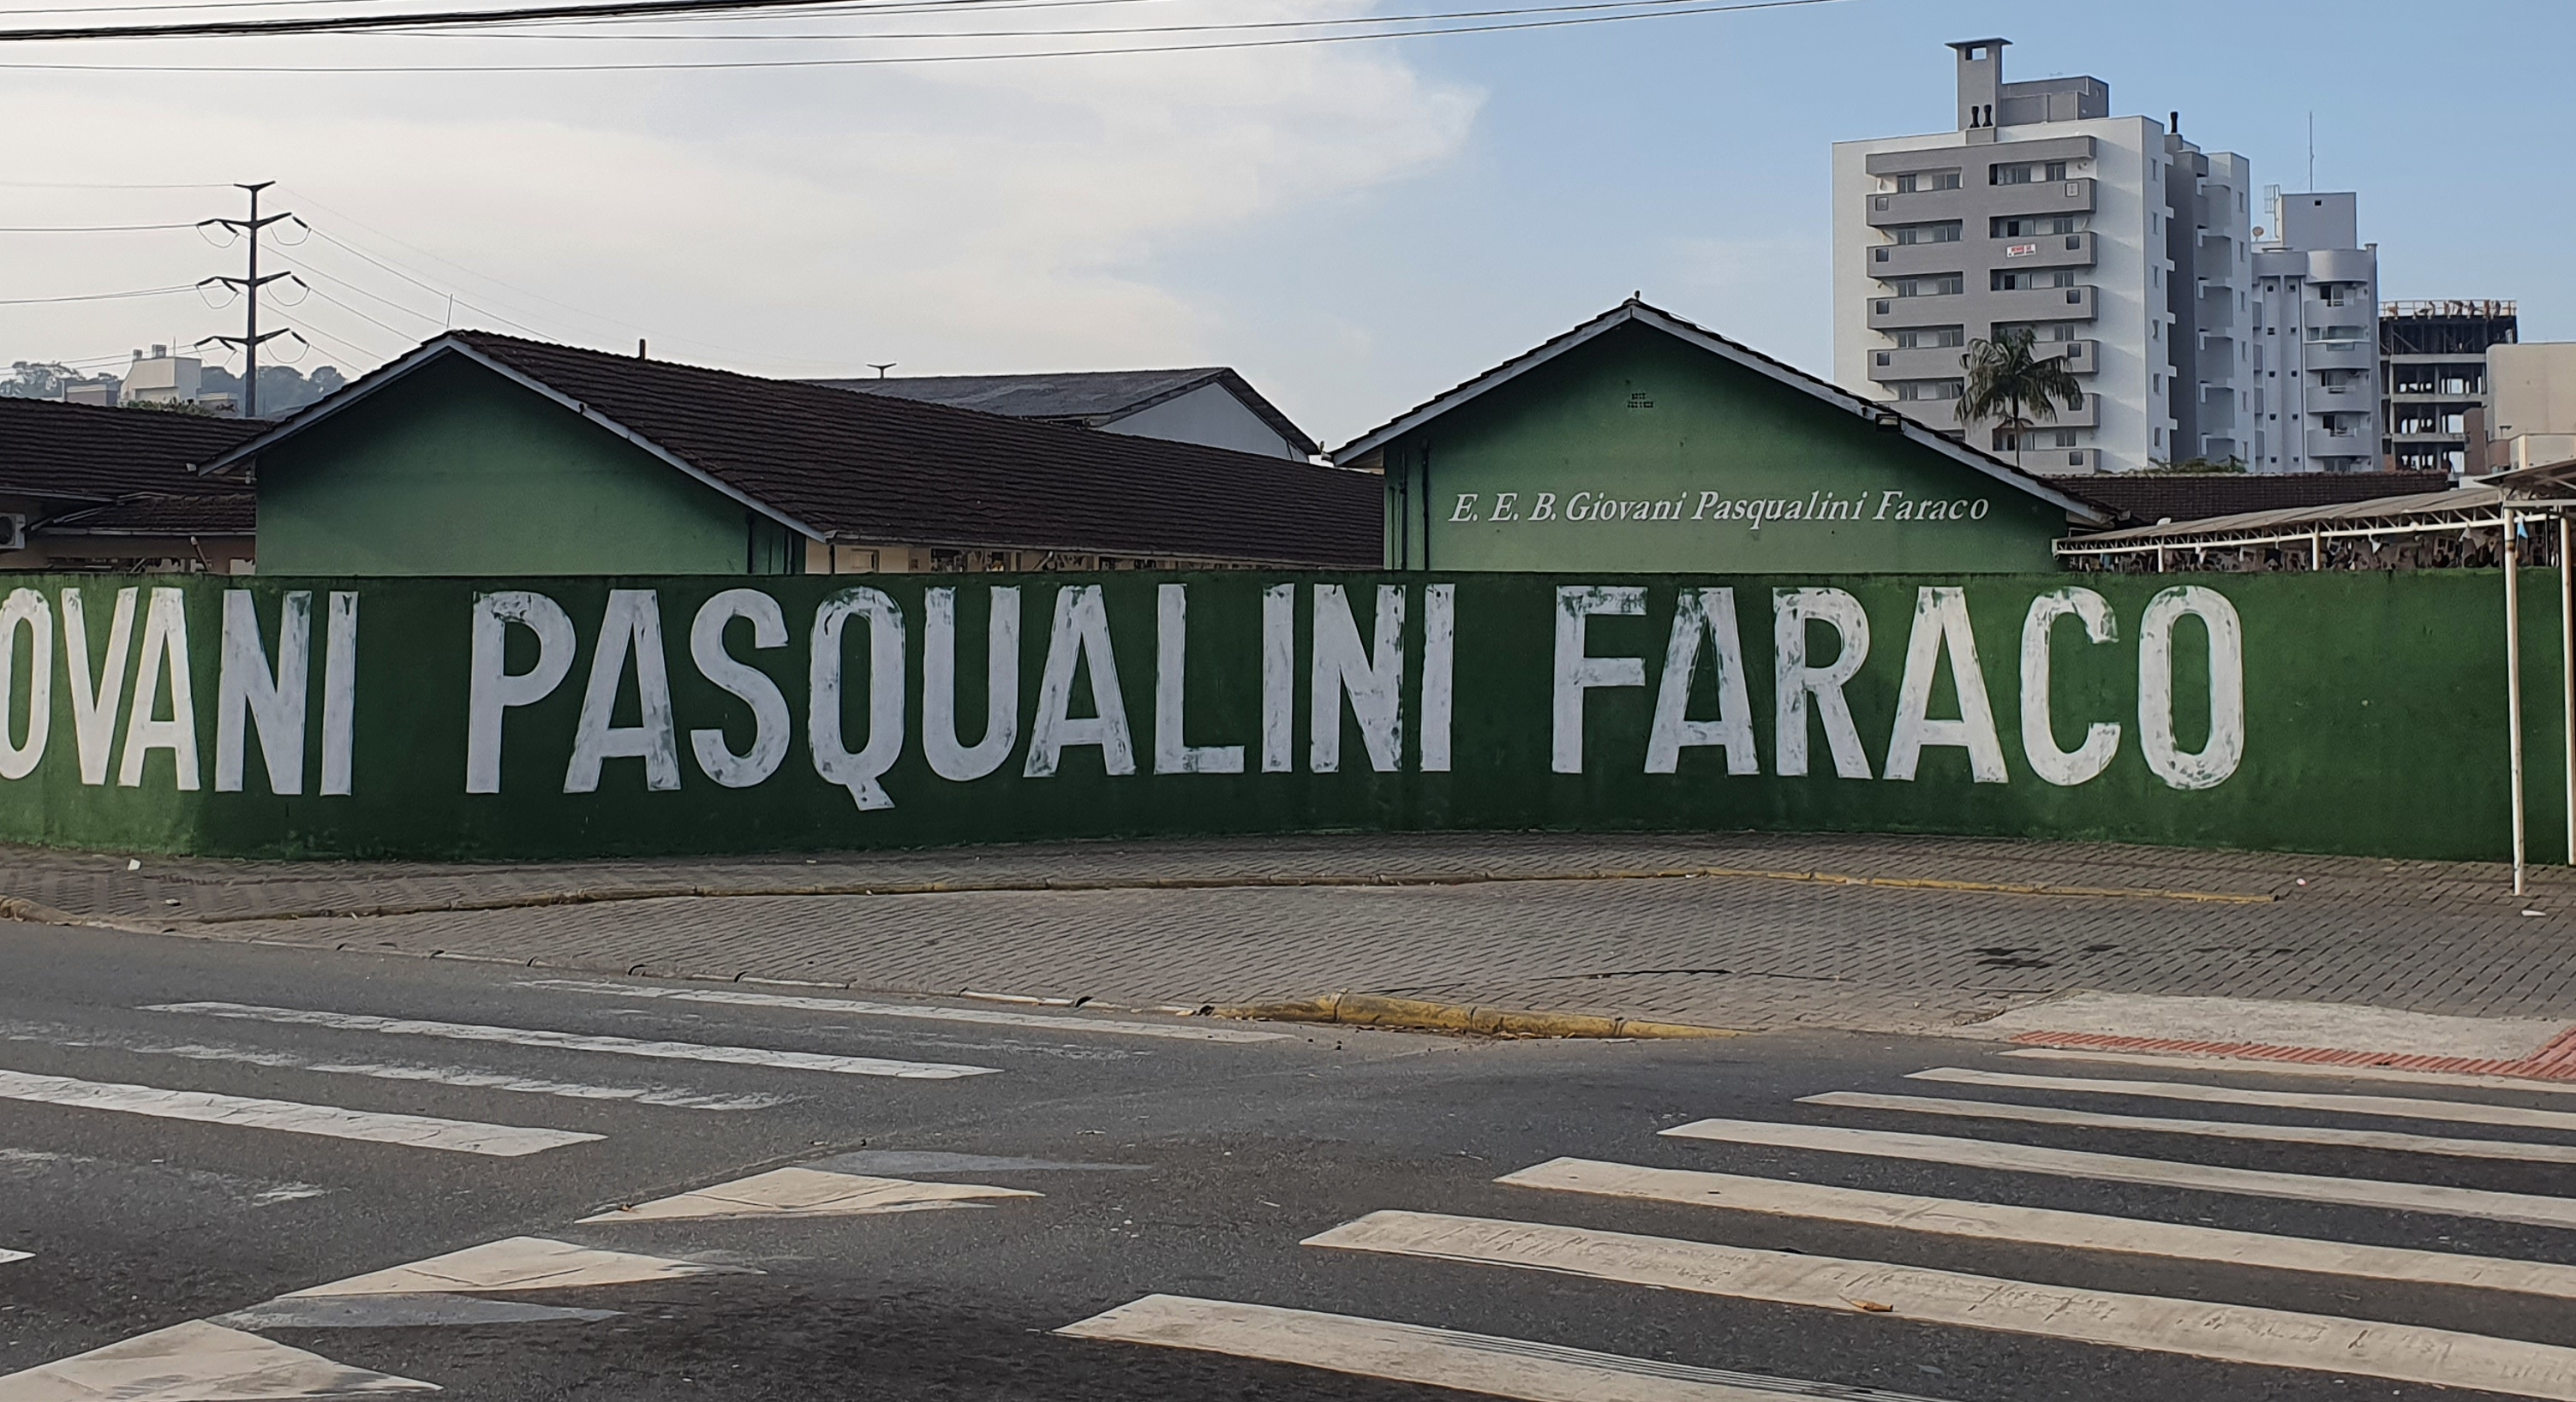
\includegraphics[width=\linewidth]{img/vista-ext01.jpg}
				\caption{Vista Externa}
			}
			\only<4>{
				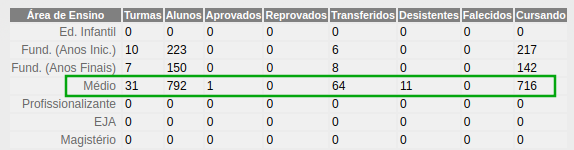
\includegraphics[width=\linewidth]{img/introducao-alunos.png}
				\caption{Fonte: Institucional}
			}
		\end{figure}
	\end{columns}
\end{frame}

\begin{frame}{Introdução}
	\framesubtitle{Infraestrutura/Apoio Docente}
	\begin{columns}
		\column{0.5\textwidth}
		\begin{itemize}
			\item Sala de Informática -- \textcolor<1>{olive}{25 CPUs Novas + 32 Tablets}
			\item<2-> Sala de \textcolor<2>{olive}{Laboratório}
			\item<3-> Salas de Aulas --  \textcolor<3>{olive}{11 Lousas Dig. p/ NEM}
			\item<4-> Quadras de Esportes -- \textcolor<4>{olive}{Coberta/Ar Livre}
		\end{itemize}

		\column{0.5\textwidth}
		\begin{figure}[htb!]
			\centering
			\only<1>{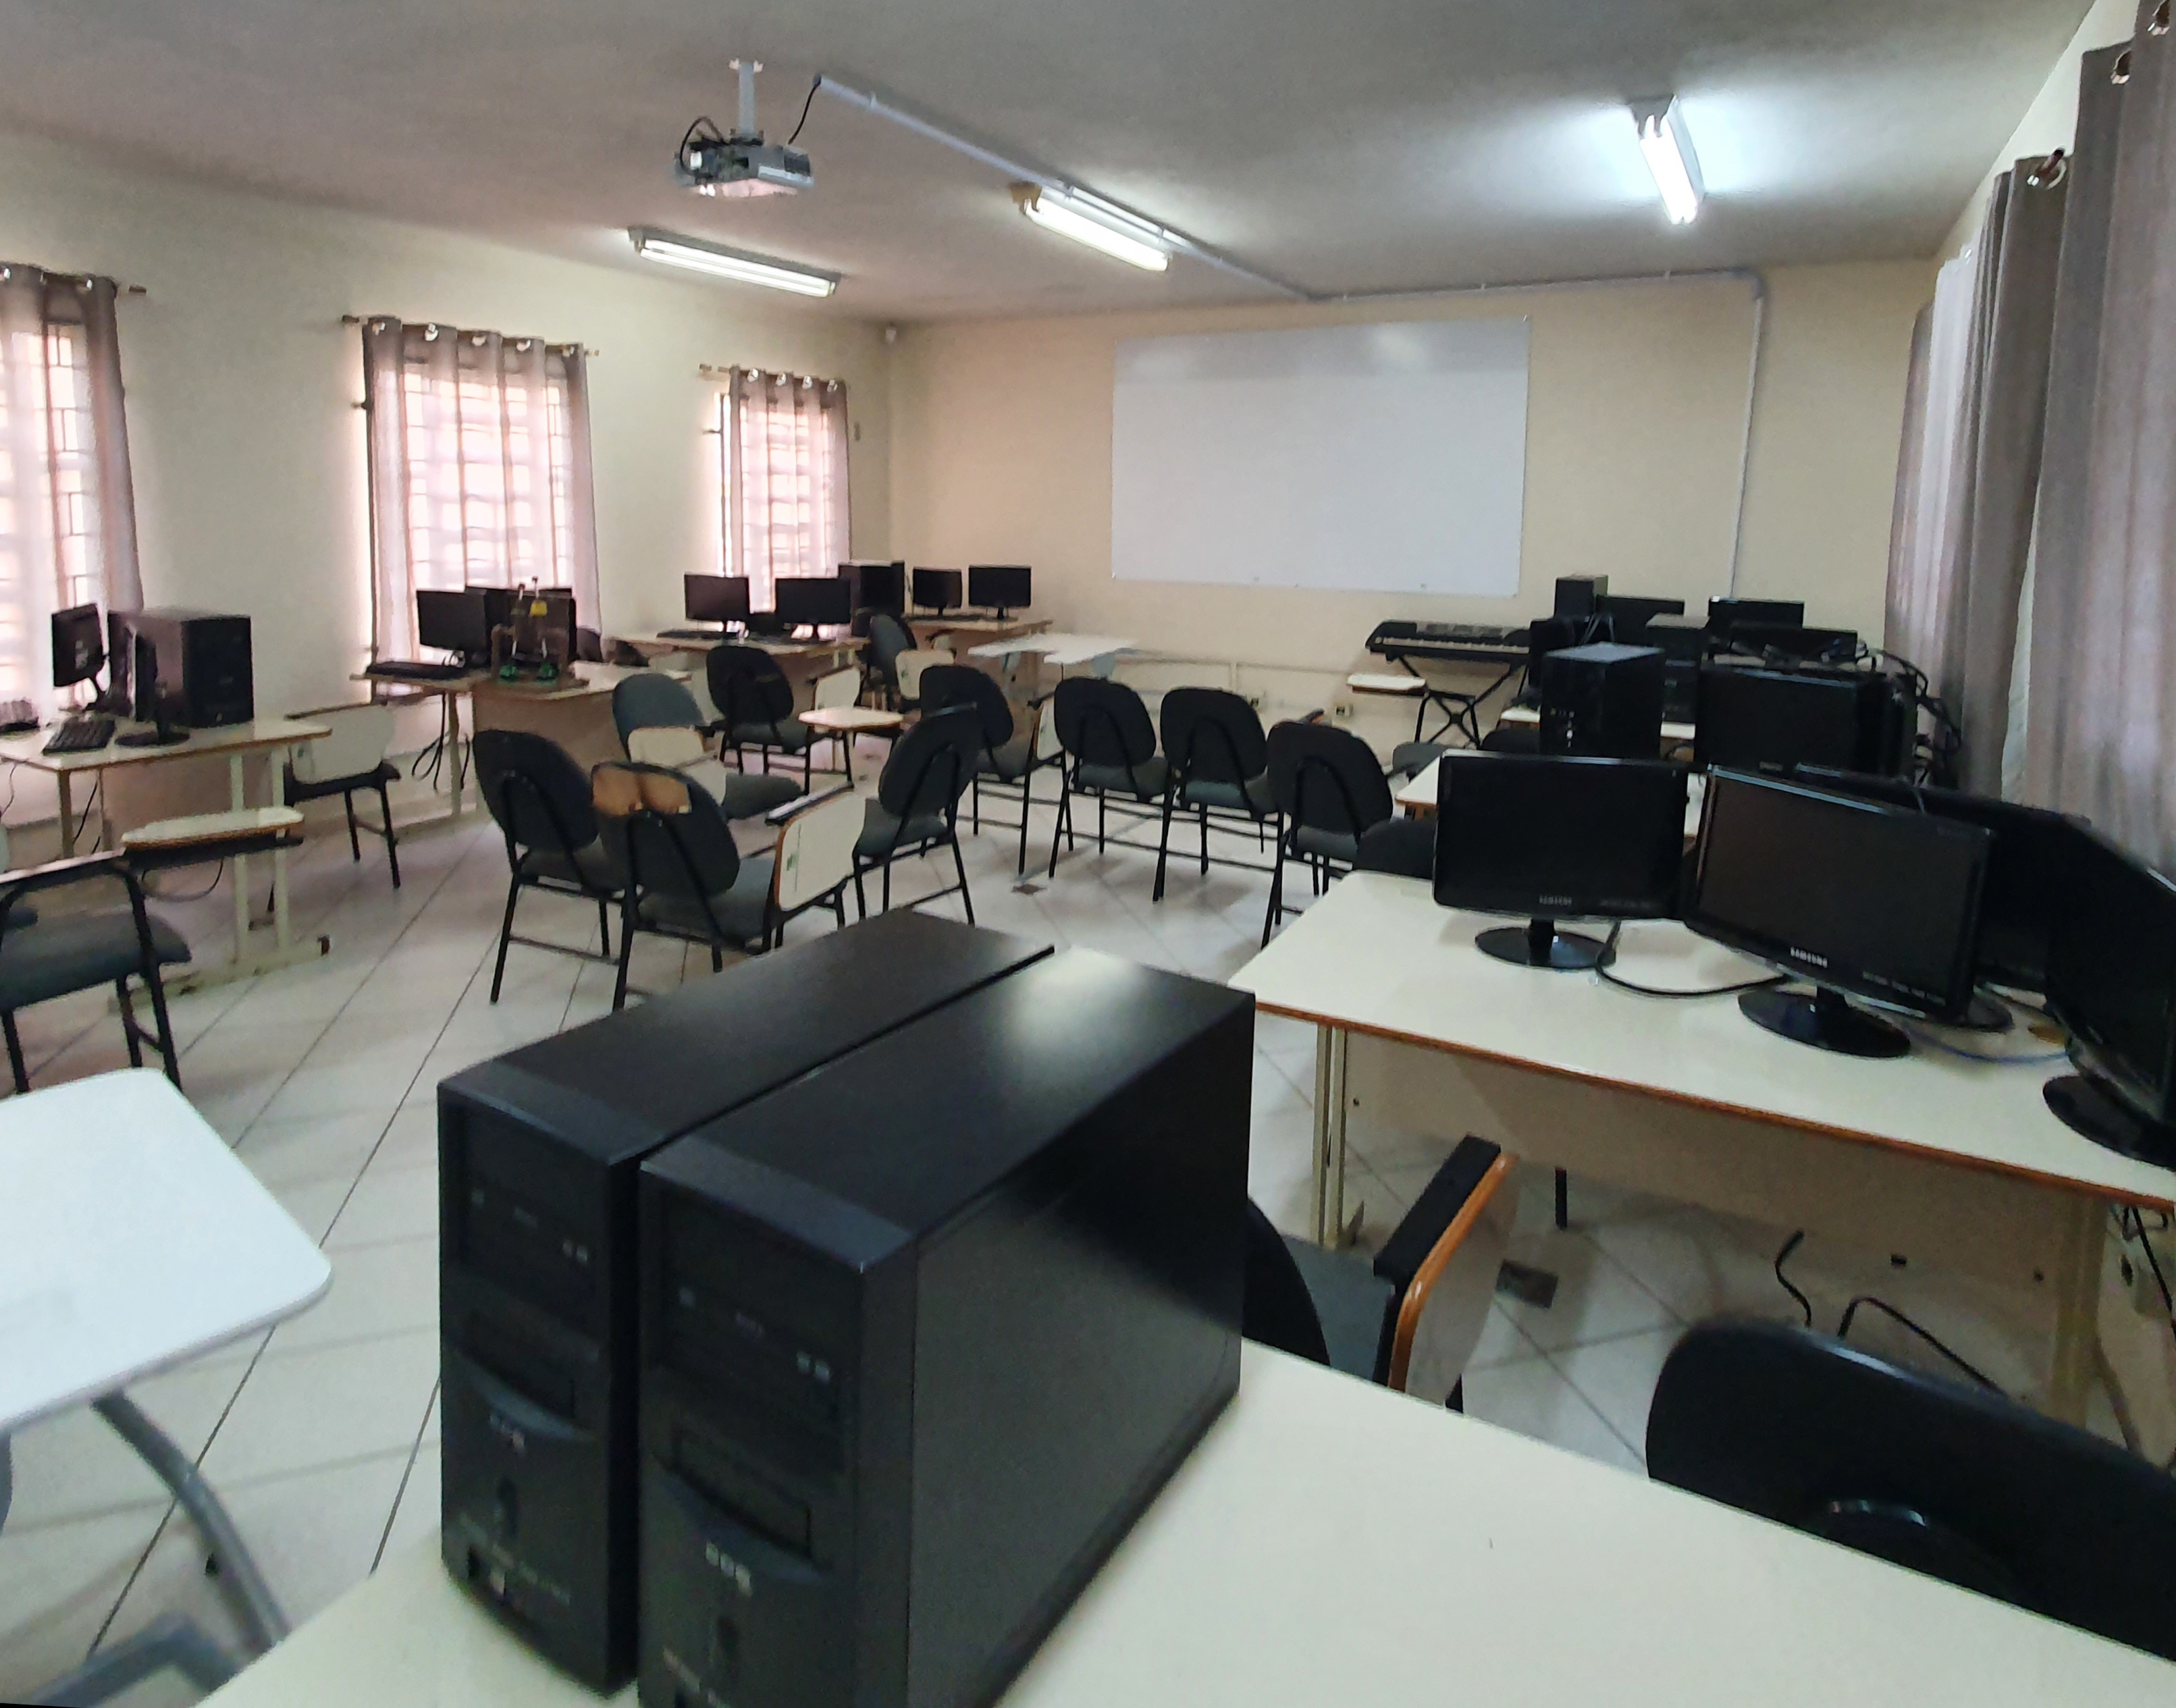
\includegraphics[width=\linewidth]{sala-de-informatica02.jpg}}
			\only<2>{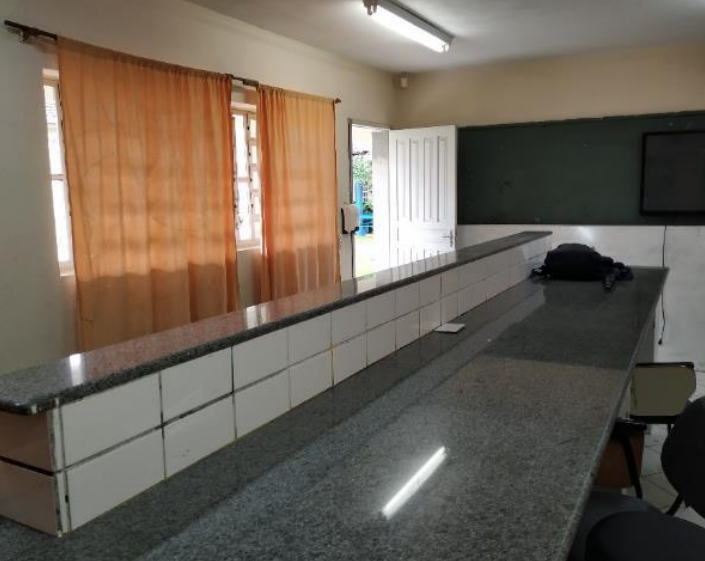
\includegraphics[width=\linewidth]{introducao-lab.png}}
			\only<3>{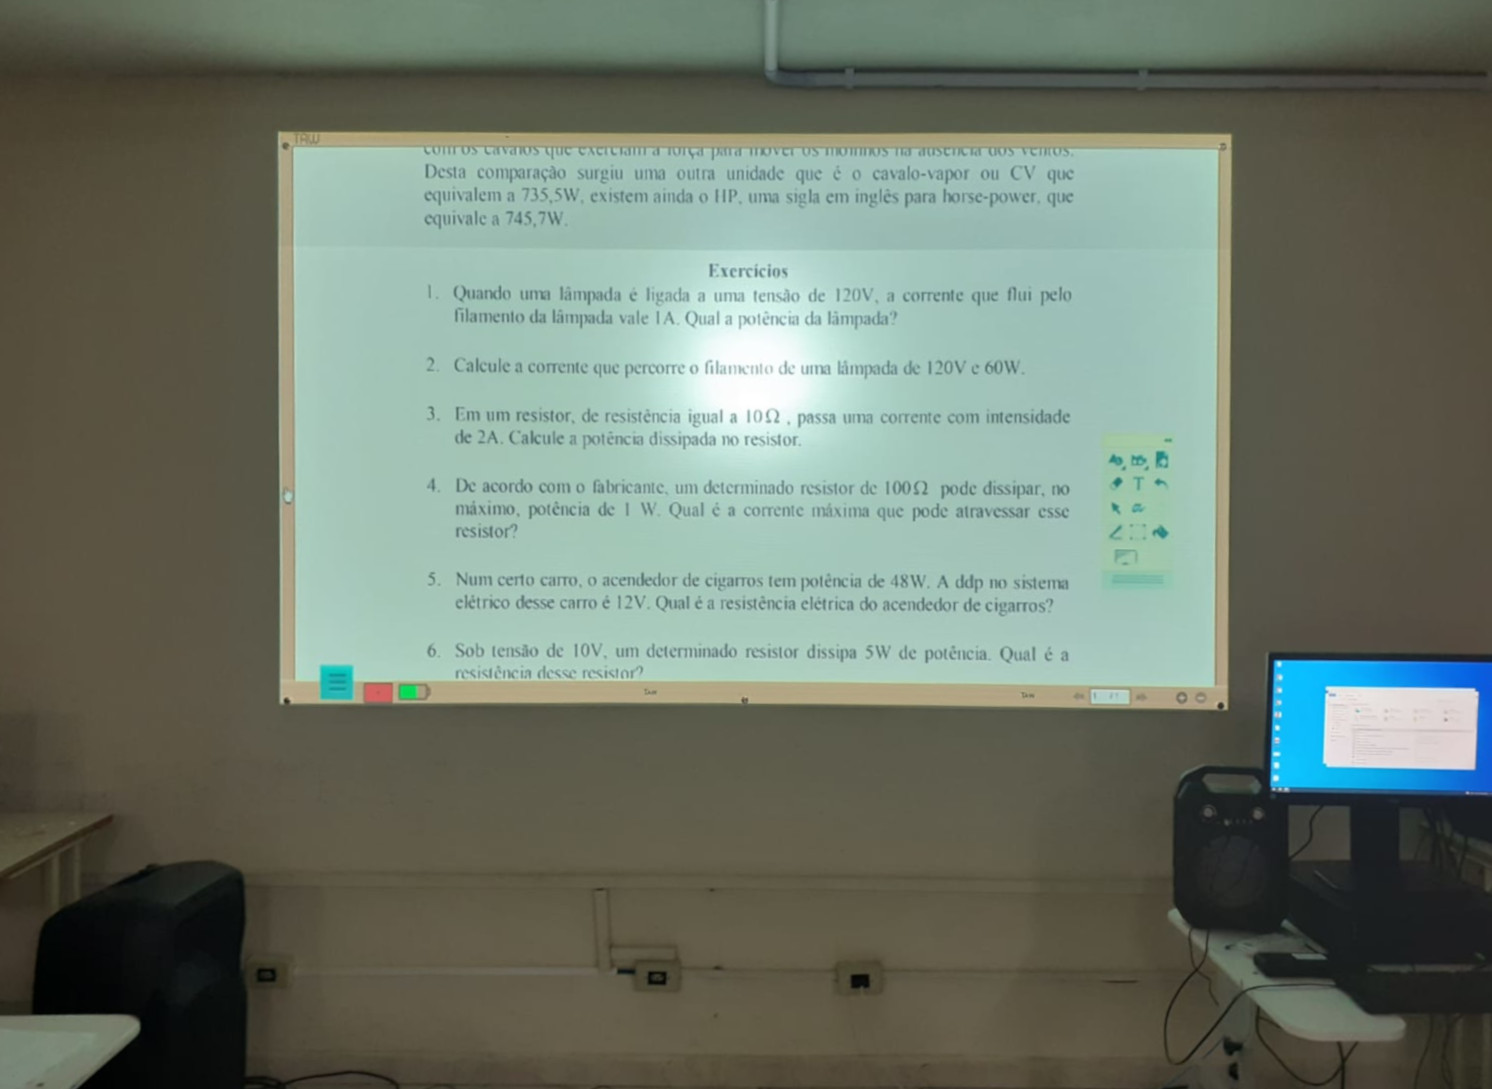
\includegraphics[width=\linewidth]{introducao-lousaD.jpeg}}
			\only<4>{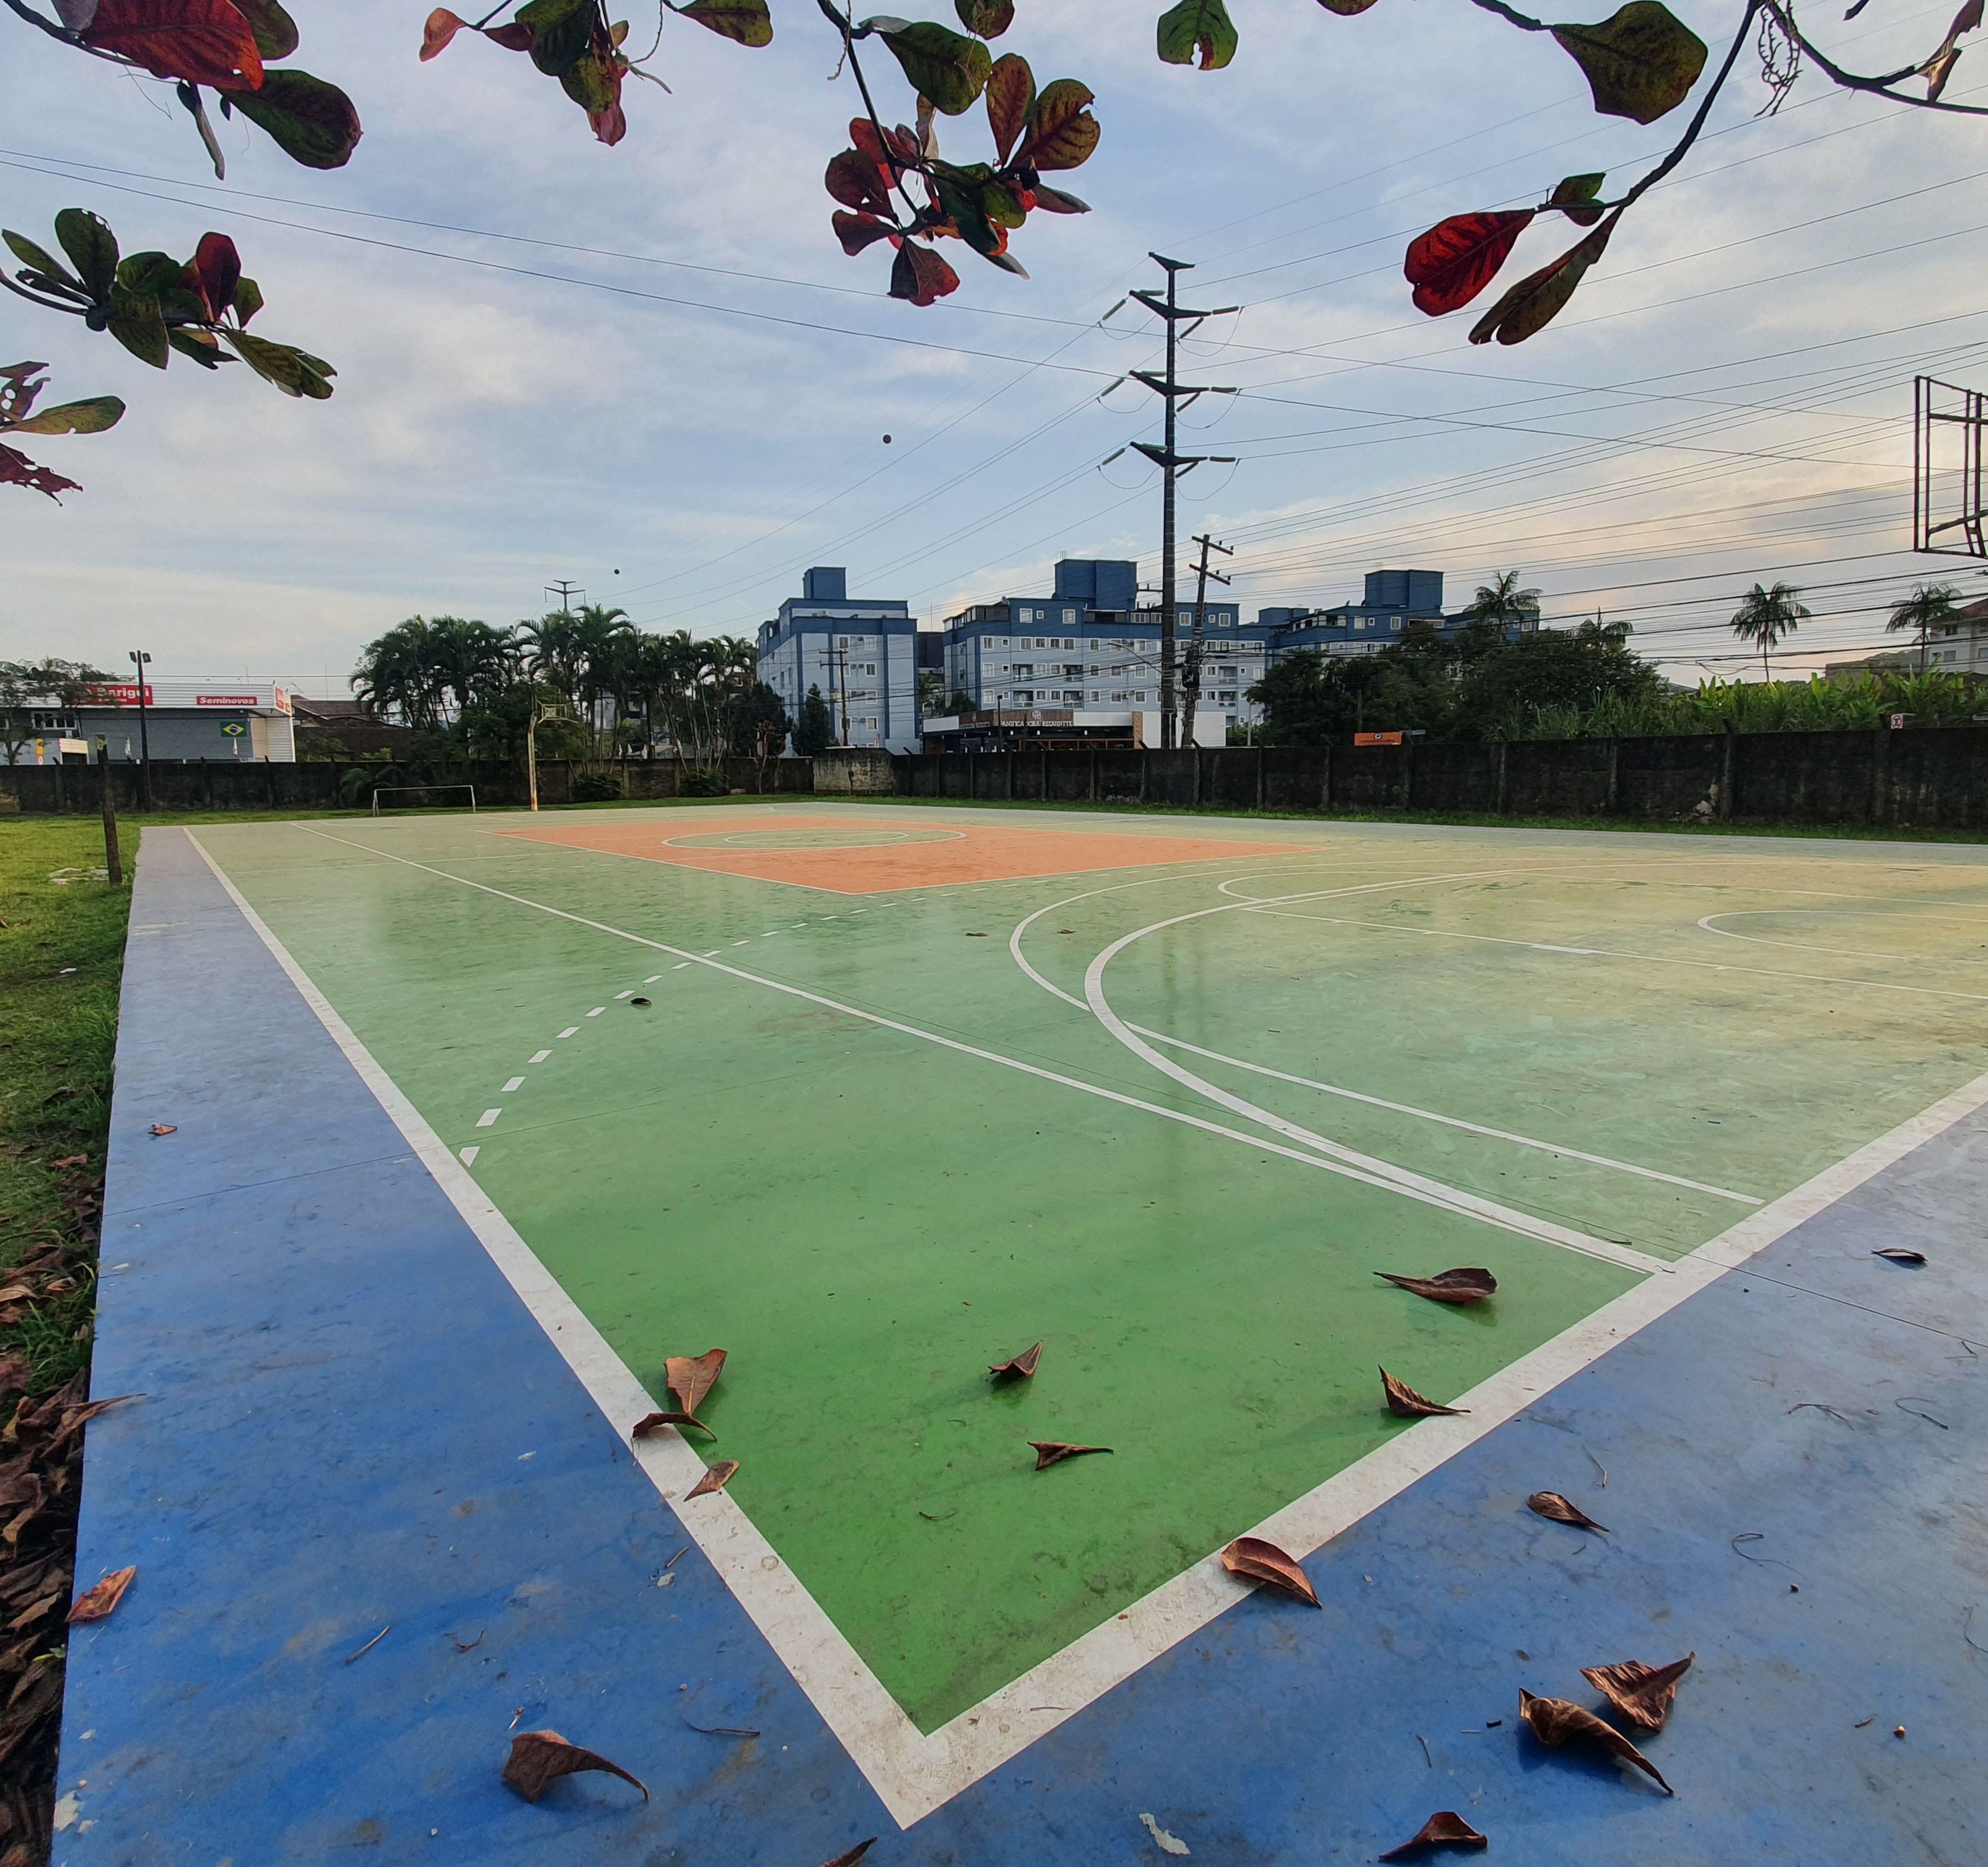
\includegraphics[width=\linewidth]{introducao-quadra.jpg}}
		\end{figure}
	\end{columns}
\end{frame}

\begin{frame}[plain]
	\tikzset{
		udesc greenBox/.style = {
			thin,
			blur shadow={
				shadow blur steps=10,
				shadow blur extra rounding=2pt, 
				shadow xshift=1pt
			},
			rectangle,
			minimum width=15em,
			minimum height=20mm,
			fill=greenudesc,
			text centered,
			anchor=base,
			inner sep=2ex
		},
	}
	\begin{tikzpicture}[remember picture,overlay]
		\node
			[udesc greenBox,yshift=-25pt,xshift=10pt] (box){}; 
		\node [right of = box, align=right,text=white] { {\LARGE Atividades de }\\Observação};
	\end{tikzpicture}
\end{frame}

\begin{frame}{Atividades de Observação}
	\framesubtitle{Aulas assistidas}
	\begin{columns}
		\column{0.5\textwidth}
		\begin{tikzpicture}
			\only<2->{
				\node [mathnode, draw, align=center, text width=3.6cm] (a1) at (0,0){
						\begin{minipage}{\textwidth}
							\centering
							Abordagens de Introdução de Conteúdo
							\cite{CARVALHO:1999}
						\end{minipage}
					};
				\only<3>{
					\node [squarednode, draw, align=center, text width=2.3cm, right=.5cm] (a2) at (a1.east){
							\begin{minipage}{\textwidth}
								\centering
								Usa situações do cotidiano do aluno
							\end{minipage}
						};

					\draw [->, line width=1pt] (a1) -- (a2);
				}
			}
			% --------------------------------------------- %
			\only<4->{
				\node [mathnode, draw, align=center, text width=3.6cm,below=.5] (a3) at (a1.south){
						\begin{minipage}{\textwidth}
							\centering
							Abordagens de Experimentais
							\cite{CARVALHO:1999}
						\end{minipage}
					};
				\only<4>{
					\node [squarednode, draw, align=center, text width=2.3cm, right=.5cm] (a4) at (a3.east){
							\begin{minipage}{\textwidth}
								\centering
								Instiga a curiosidade dos alunos
							\end{minipage}
						};

					\draw [->, line width=1pt] (a3) -- (a4);
				}
			}
			% --------------------------------------------- %
			\only<5>{
				\node [mathnode, draw, align=center, text width=3.6cm,below=.5] (a5) at (a3.south){
						\begin{minipage}{\textwidth}
							\centering
							Abordagens de Exercícios
							\cite{PEREZ:1992}
						\end{minipage}
					};
				\only<5>{
					\node [squarednode, draw, align=center, text width=2.3cm, right=.5cm] (a6) at (a5.east){
							\begin{minipage}{\textwidth}
								\centering
								Trabalha o Domínio Conceitual
							\end{minipage}
						};

					\draw [->, line width=1pt] (a5) -- (a6);
				}
			}
		\end{tikzpicture}

		\column{0.5\textwidth}
		\begin{table}
			\centering
			\resizebox{\linewidth}{!}{%
				\begin{tabular}{|r|c|l|}
					\hline
					\multicolumn{1}{|c|}{\textbf{Data}} & \textbf{Turma} & \multicolumn{1}{c|}{\textbf{Assunto}} \\ \hline
					\textbf{22/03} & \textbf{3(4)} & \textcolor<5->{olive}{Lei de Coulomb (Exercícios)}                  \\ \hline
					\textbf{}      & \textbf{2(6)} & \textcolor<5->{olive}{Calorimetria (Exercícios)}                    \\ \hline
					\textbf{}      & \textbf{2(6)} & \textcolor<5->{olive}{Calorimetria (Revisão)}                       \\ \hline
					\textbf{24/03} & \textbf{3(4)} & \textcolor<2->{olive}{Corrente Elétrica (Introdução)}               \\ \hline
					\textbf{}      & \textbf{2(6)} & \textcolor<5->{olive}{Calorimetria (Avaliação)}                     \\ \hline
					\textbf{}      & \textbf{2(6)} & \textcolor<5->{olive}{Calorimetria (Correção)}                      \\ \hline
					\textbf{31/03} & \textbf{1(5)} & \textcolor<2->{olive}{Movimento Retilíneo Uniforme (Introdução)}    \\ \hline
					\textbf{}      & \textbf{2(6)} & \textcolor<4->{olive}{Dilatação Térmica (Exp. Demostrativo)}        \\ \hline
					\textbf{05/05} & \textbf{3(4)} & \textcolor<5->{olive}{Corrente Elétrica (Revisão)}                  \\ \hline
					\textbf{}      & \textbf{1(5)} & \textcolor<2->{olive}{Vetores (Introdução)}                         \\ \hline
				\end{tabular}%
			}
			\caption{Acompanhamento de aulas}
			\label{tab:acompanhamento-aulas}
		\end{table}
	\end{columns}
\end{frame}
% --------------------------------------------- %
\begin{frame}{Reuniões Pedagógicas}
\framesubtitle{Conselho de Classe}
\begin{alertblock}{Conselho de Classe}
	Principais pontos discutidos:
	\only<2->{
		\begin{itemize}
				\item<2-> Data: 08/05 às 18h;
				\item<3-> Casos de Dengue
				\item<4-> Notas/comportamento/faltas;
				\item<5-> 2(6) foi citado.
		\end{itemize}
	}
\end{alertblock}	
\end{frame}


\begin{frame}{Reuniões Pedagógicas}
\framesubtitle{Estatísticas}
\begin{columns}
	\column{0.5\textwidth}
	\begin{figure}[htb!]
		\centering
		\only<1>{
			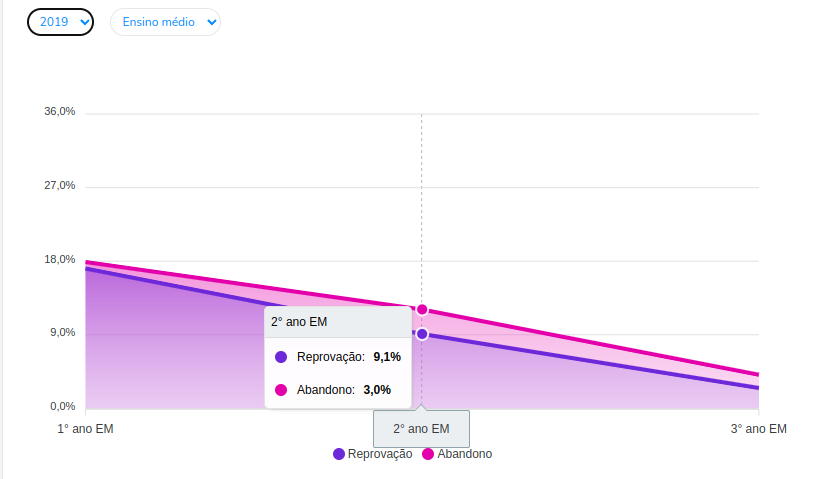
\includegraphics[width=\linewidth]{estatistica-2019.png}
			\caption{Taxas de rendimento escolar (GPF) -- Fonte: INEP 2019}
		}
		\only<2>{
			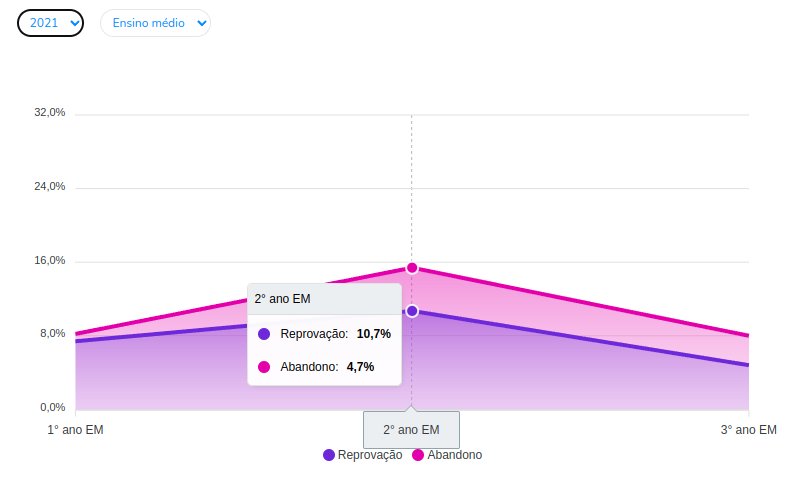
\includegraphics[width=\linewidth]{estatistica-2021.png}
			\caption{Taxas de rendimento escolar (GPF) -- Fonte: INEP 2021}
		}
	\end{figure}

	\column{0.5\textwidth}
	\begin{figure}[htb!]
		\centering
		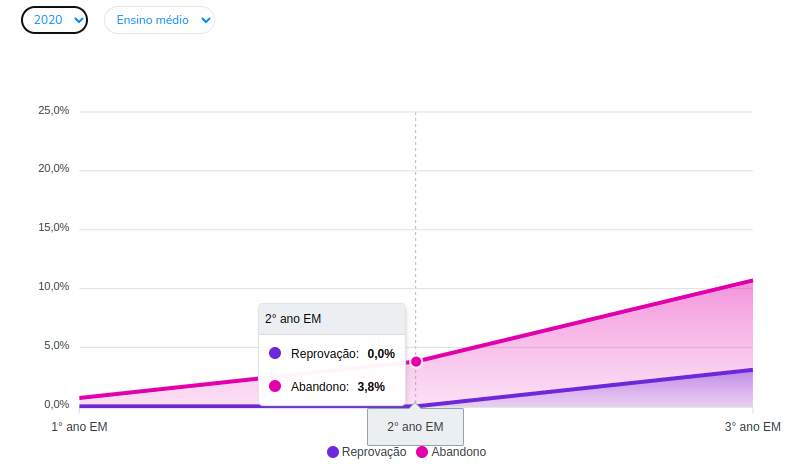
\includegraphics[width=\linewidth]{estatistica-2020.png}
			\caption{Taxas de rendimento escolar (GPF) -- Fonte: INEP 2020}
	\end{figure}

\end{columns}
\end{frame}



% --------------------------------------------- %
\begin{frame}[plain]
	\tikzset{
		udesc greenBox/.style = {
			thin,
			blur shadow={
				shadow blur steps=10,
				shadow blur extra rounding=2pt, 
				shadow xshift=1pt
			},
			rectangle,
			minimum width=15em,
			minimum height=20mm,
			fill=greenudesc,
			text centered,
			anchor=base,
			inner sep=2ex
		},
	}
	\begin{tikzpicture}[remember picture,overlay]
		\node
			[udesc greenBox,yshift=-25pt,xshift=10pt] (box){}; 
		\node [right of = box, align=right,text=white] { {\LARGE Atividades de }\\Regência};
	\end{tikzpicture}
\end{frame}
\begin{frame}{Atividades de Regência}
\framesubtitle{Perfil da Turma}
\begin{columns}
	\column{0.5\textwidth}
	\begin{itemize}
		\item 36 Alunos/($18\sim20$ comparecem)
		\item $\langle t \rangle = 17$ anos
		\item Temperamento: Quietos
	\end{itemize}

	\column{0.5\textwidth}
	\begin{figure}[htb!]
		\centering
		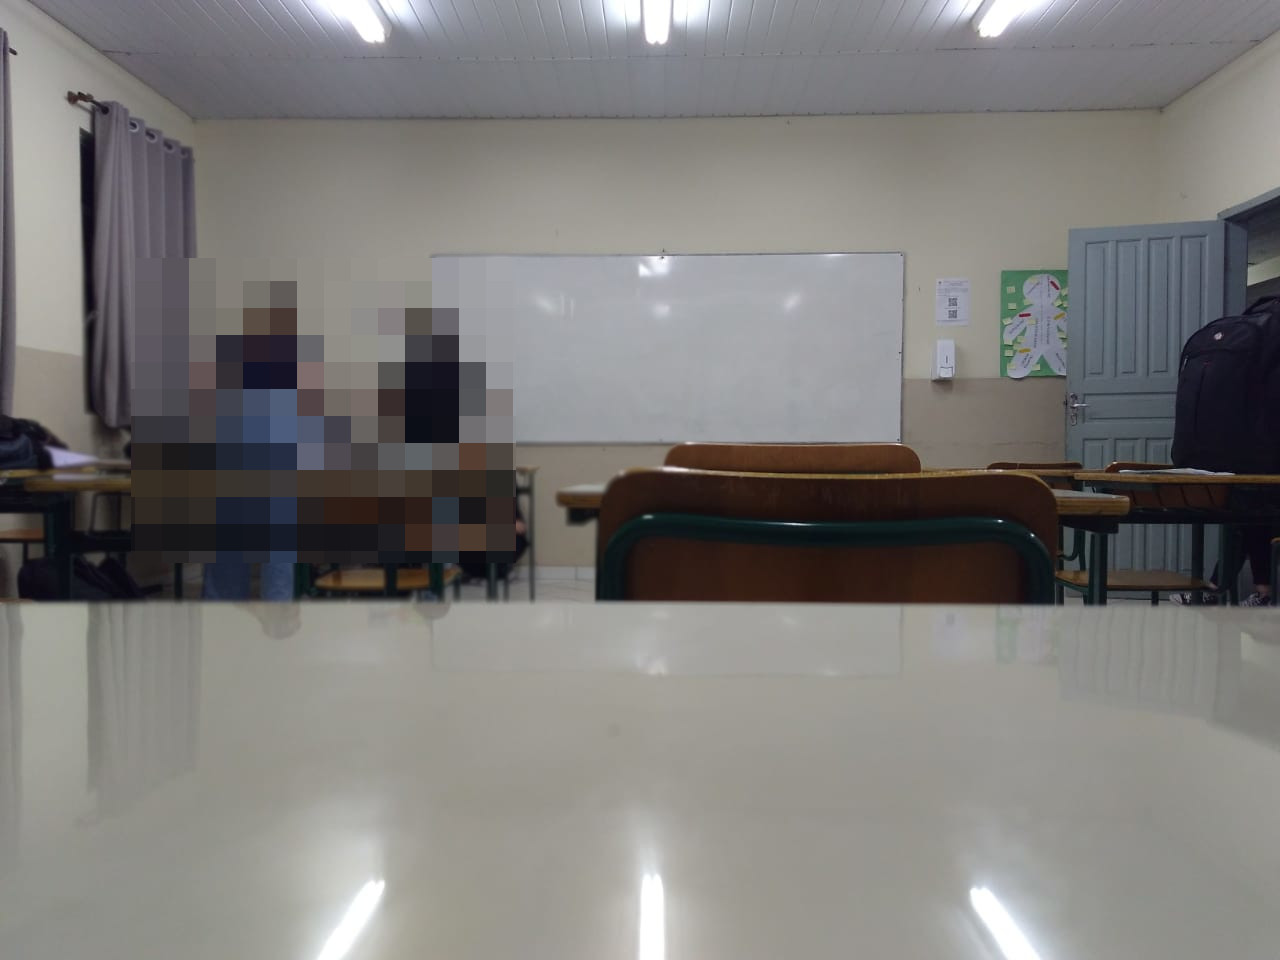
\includegraphics[width=\linewidth]{perfil-turma.jpeg}
	\end{figure}
\end{columns}
\end{frame}

\begin{frame}{Trilha}
\framesubtitle{Carga Horária}
\begin{figure}[htb!]
	\centering
	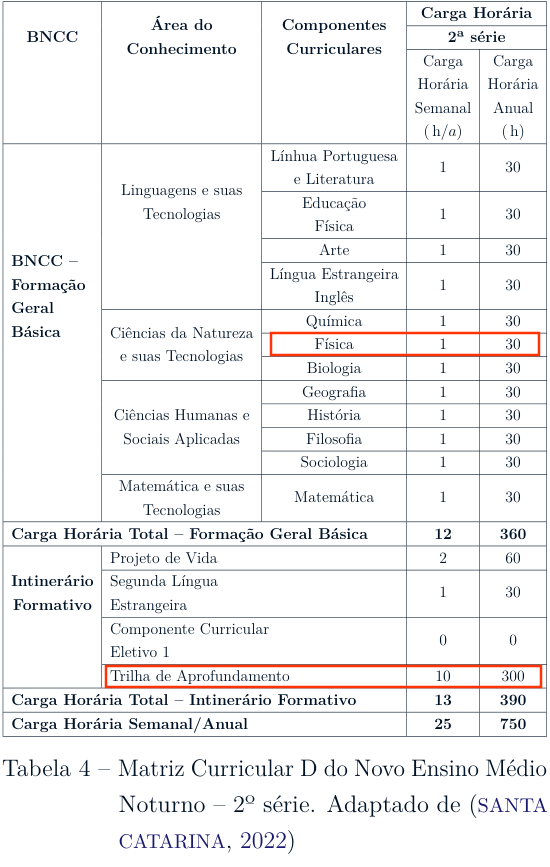
\includegraphics[width=.3\linewidth]{carga-horariaNEM.png}
\end{figure}	
\end{frame}

\begin{frame}{Trilha}
\framesubtitle{Aspectos Gerais}
\begin{figure}[htb!]
	\centering
	\only<1>{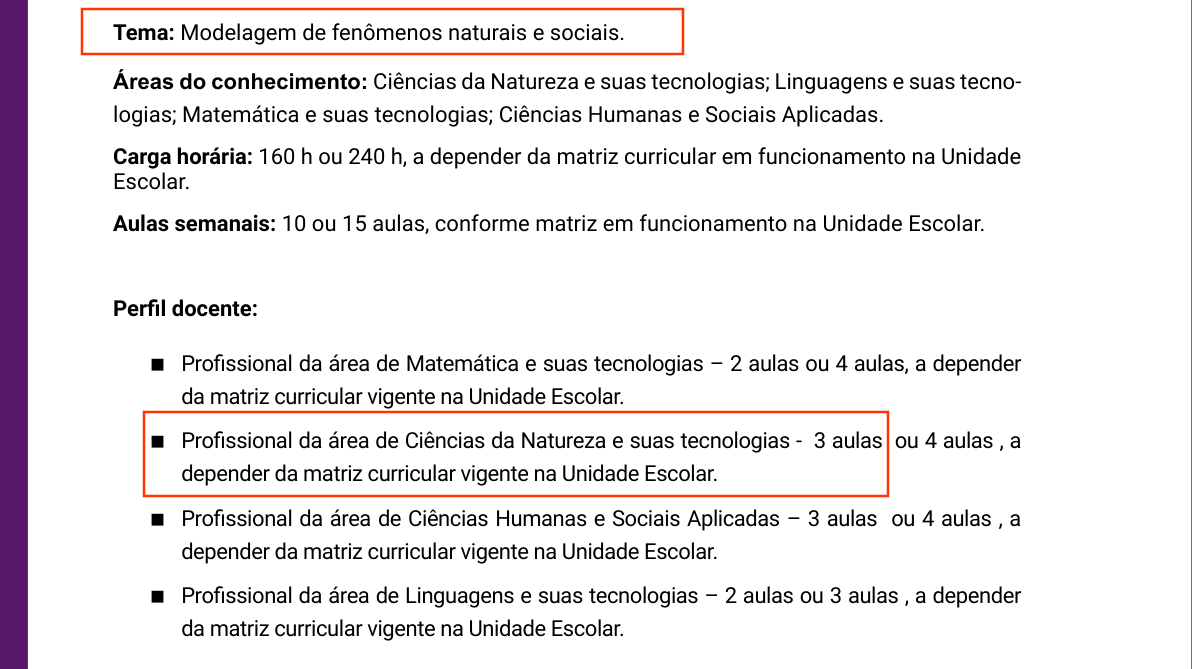
\includegraphics[width=.7\linewidth]{trilha-01.png}}
	\only<2>{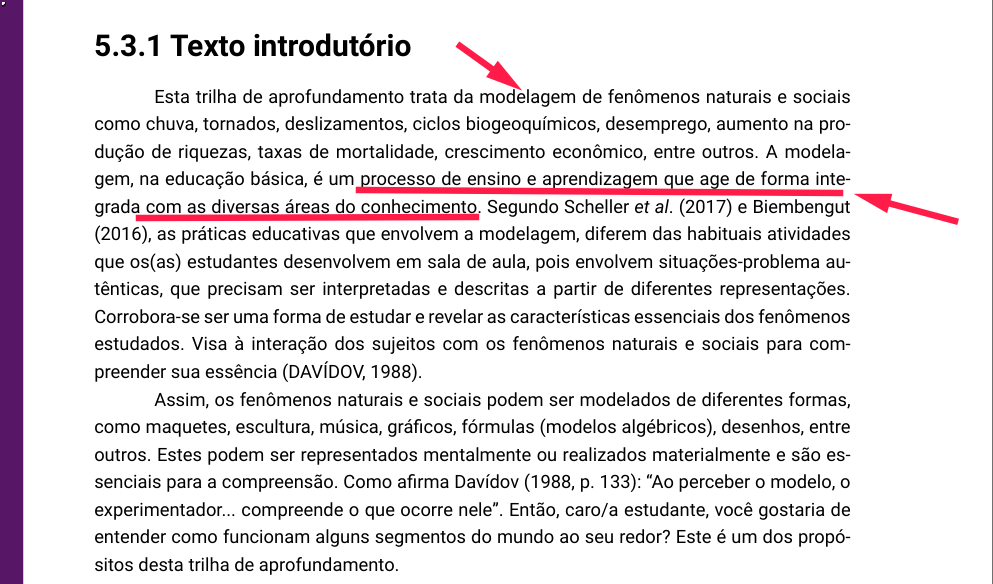
\includegraphics[width=.7\linewidth]{trilha-objetivos.png}}
	\only<3>{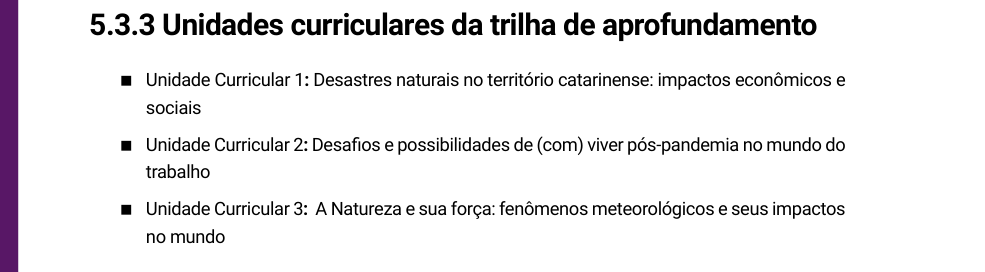
\includegraphics[width=.5\linewidth]{trilha-unidades.png}}
	\only<4>{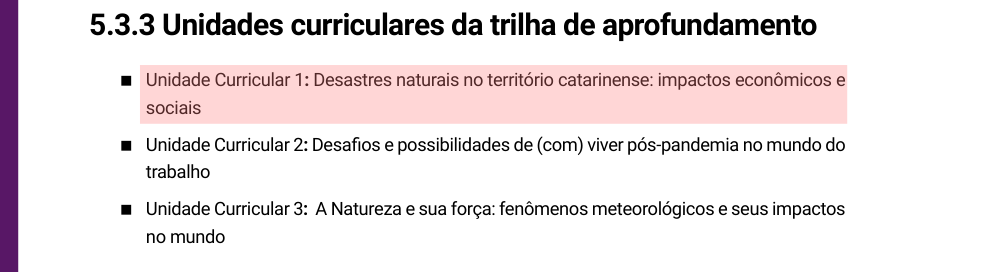
\includegraphics[width=.5\linewidth]{trilha-unidades2.png}}
	\only<4>{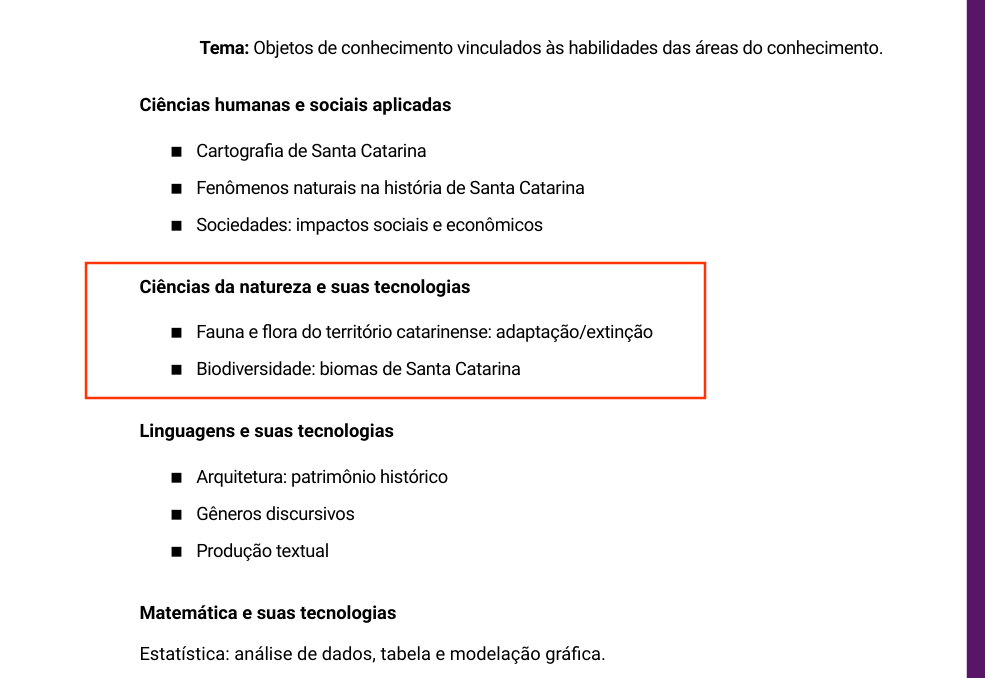
\includegraphics[width=.5\linewidth]{trilha-uniObjetivos.png}}
\end{figure}	
\end{frame}

\begin{frame}{Planejamento}
\framesubtitle{Sequência Didática}
\begin{columns}
	\column{0.4\textwidth}
	\begin{alertblock}{Planejamento}
		Metodologia Dialética \cite{VASCONCELLOS:1992}
		\begin{itemize}
			\item<1-> Total de 10 aulas (dias: quartas e sextas)
			\item<2-> \textcolor<2>{red}{Síncrese} (Construção do conhecimento)
			\item<3-> \textcolor<3>{red}{Análise} (Eslaboração da sítese)
			\item<4-> \textcolor<4>{red}{Síntese} (Síntese do conhecimento)
		\end{itemize}
	\end{alertblock}
	

	\column{0.6\textwidth}
	\begin{figure}[htb!]
		\centering
		\only<1>{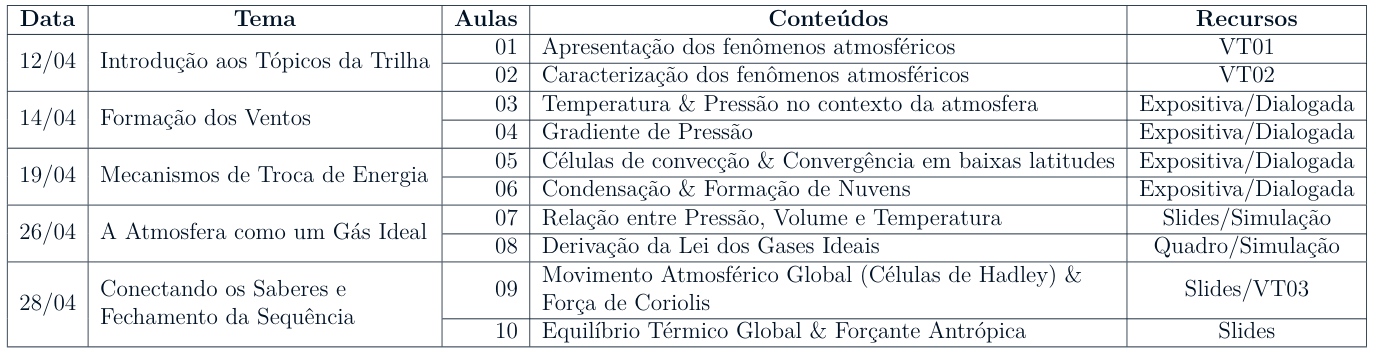
\includegraphics[width=\linewidth]{planejamento-01.png}}
		\only<2>{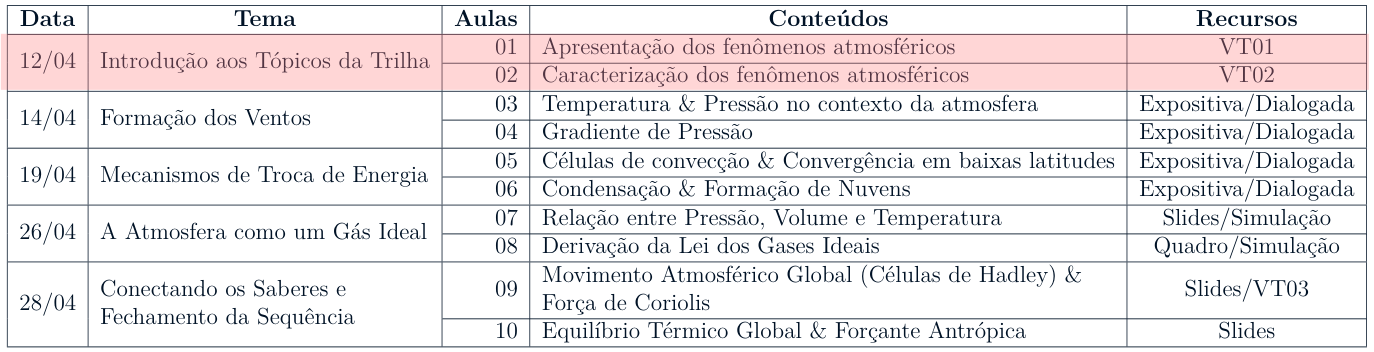
\includegraphics[width=\linewidth]{planejamento-02.png}}
		\only<3>{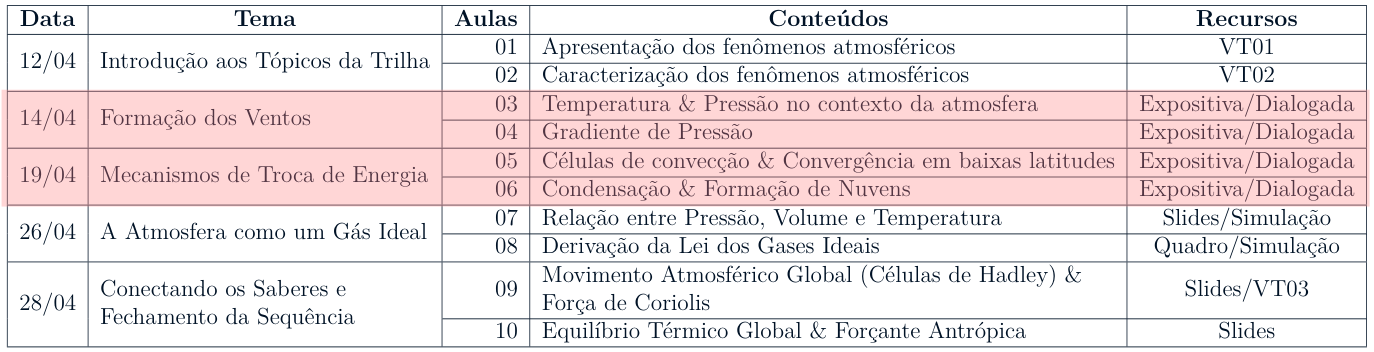
\includegraphics[width=\linewidth]{planejamento-03.png}}
		\only<4>{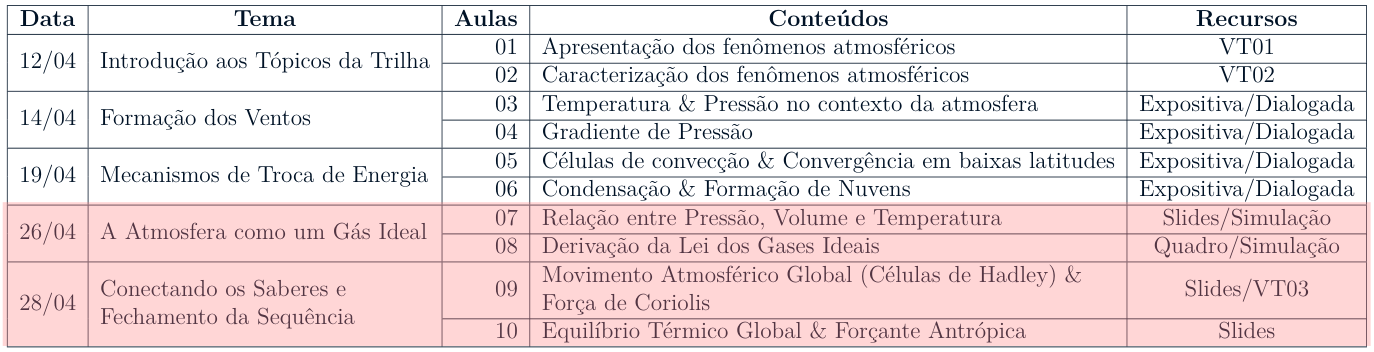
\includegraphics[width=\linewidth]{planejamento-04.png}}
	\end{figure}
\end{columns}
\end{frame}

\begin{frame}{Análises}
\framesubtitle{SEI}
	\only<1>{
		\begin{alertblock}{Pontos Positivos}
			\begin{itemize}
					\item Tema/Trilha $\to$ Abrangente;
					\item Metodologia $\to$ Pertinente ao tema tem potencial de promover engajamentos nas aulas \cite{MARIO:2017}; 
					\item Materiais utilizados $\to$ vídeos curtos performaram bem em mantê-los a atentos;
			\end{itemize}				
		\end{alertblock}
	}
	\only<2>{
		\begin{alertblock}{Pontos Negativos}
			\begin{itemize}
					\item Tema/Trilha $\to$ Difícil de abordar, necessita muita preparação;
					\item Metodologia $\to$ Pertinente ao tema porém precisa diversificar as abordagens no decorrer da sequência;
					\item Materiais utilizados $\to$ Limitado, precisa produzir;
			\end{itemize}				
		\end{alertblock}
	}
\end{frame}

\begin{frame}{Considerações Finais}
	\only<2>{
		\begin{center}
			\huge
			\textcolor{greenudesc}{Obrigado!}
		\end{center}
	}
\end{frame}

% --------------------------------------------- %
% \begin{tikzpicture}
% 	\node [squarednode, draw, align=center, text width=3.6cm, below=2.5cm] (txt) at (0,0){
% 			\begin{minipage}{\textwidth}
% 				\centering
% 				Este aumento é ainda mais significatico para o processo $J/\psi$
% 			\end{minipage}
% 		};
% 	\node [mathnode, draw, align=center, text width=3.6cm, above=.5cm] (txt2) at (txt.north){
% 			\begin{minipage}{\textwidth}
% 				\centering
% 				Este aumento é ainda mais significatico para o processo $J/\psi$
% 			\end{minipage}
% 		};
% 	\draw [->, line width=1pt] (txt) -- (txt2);
% \end{tikzpicture}

% --------------------------------------------- %
\begin{frame}[allowframebreaks]
	\frametitle{Referências}
	\bibliography{referencias.bib}
\end{frame}

\contato{%
	Contato: \\
	\autor{} \\
	\email{} \\
	\github{} \\
	\website{}
}

\capadetras{}

\end{document}
